\subsection{Konfigurasi \textit{Deployment} Kluster Sistem Tiket}

\subsubsection{Sistem Pengawasan}

Diagram deployment untuk sistem pengawasan ditunjukkan pada Gambar \ref{fig:deployment-monitoring}. Arsitektur ini menunjukkan bagaimana Prometheus mengumpulkan metrik, sementara Loki (yang dipecah menjadi beberapa komponen seperti distributor dan ingester) mengagregasi log. Kedua sumber data ini disimpan dalam Persistent Volume Claims (pvc-storage-loki), dan Grafana berfungsi sebagai antarmuka terpadu untuk visualisasi dasbor dan log, yang diakses melalui service grafana.

\begin{figure}[H]
    \centering
    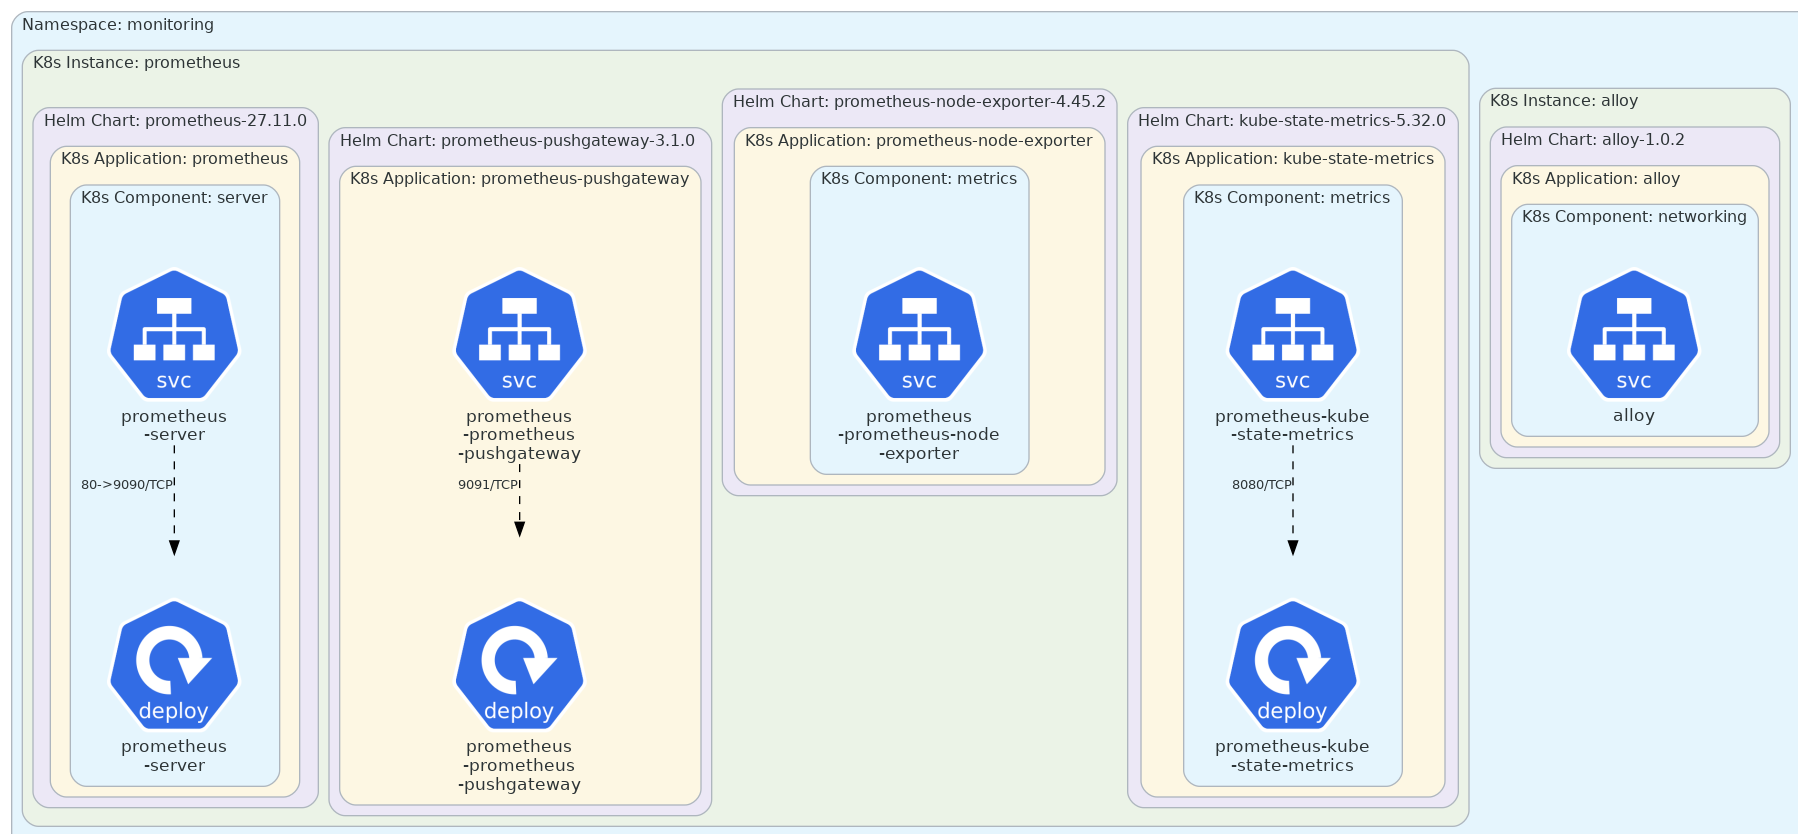
\includegraphics[width=0.9\textwidth]{resources/chapter-4/monitoring-1.png}
    \caption{\textit{Deployment} Sistem Pengawasan}
    \label{fig:deployment-monitoring}
\end{figure}

\pagebreak

\subsubsection{Nginx Ingress Controller}

Gambar \ref{fig:deployment-nginx} menampilkan arsitektur ingress. Komponen inti adalah nginx-ingress-controller, yang bertindak sebagai reverse proxy untuk mengarahkan lalu lintas eksternal ke layanan internal yang sesuai. Diagram ini juga menunjukkan integrasi dengan cert-manager yang secara otomatis mengelola sertifikat TLS untuk mengamankan endpoint yang diekspos.

\begin{figure}[H]
    \centering
    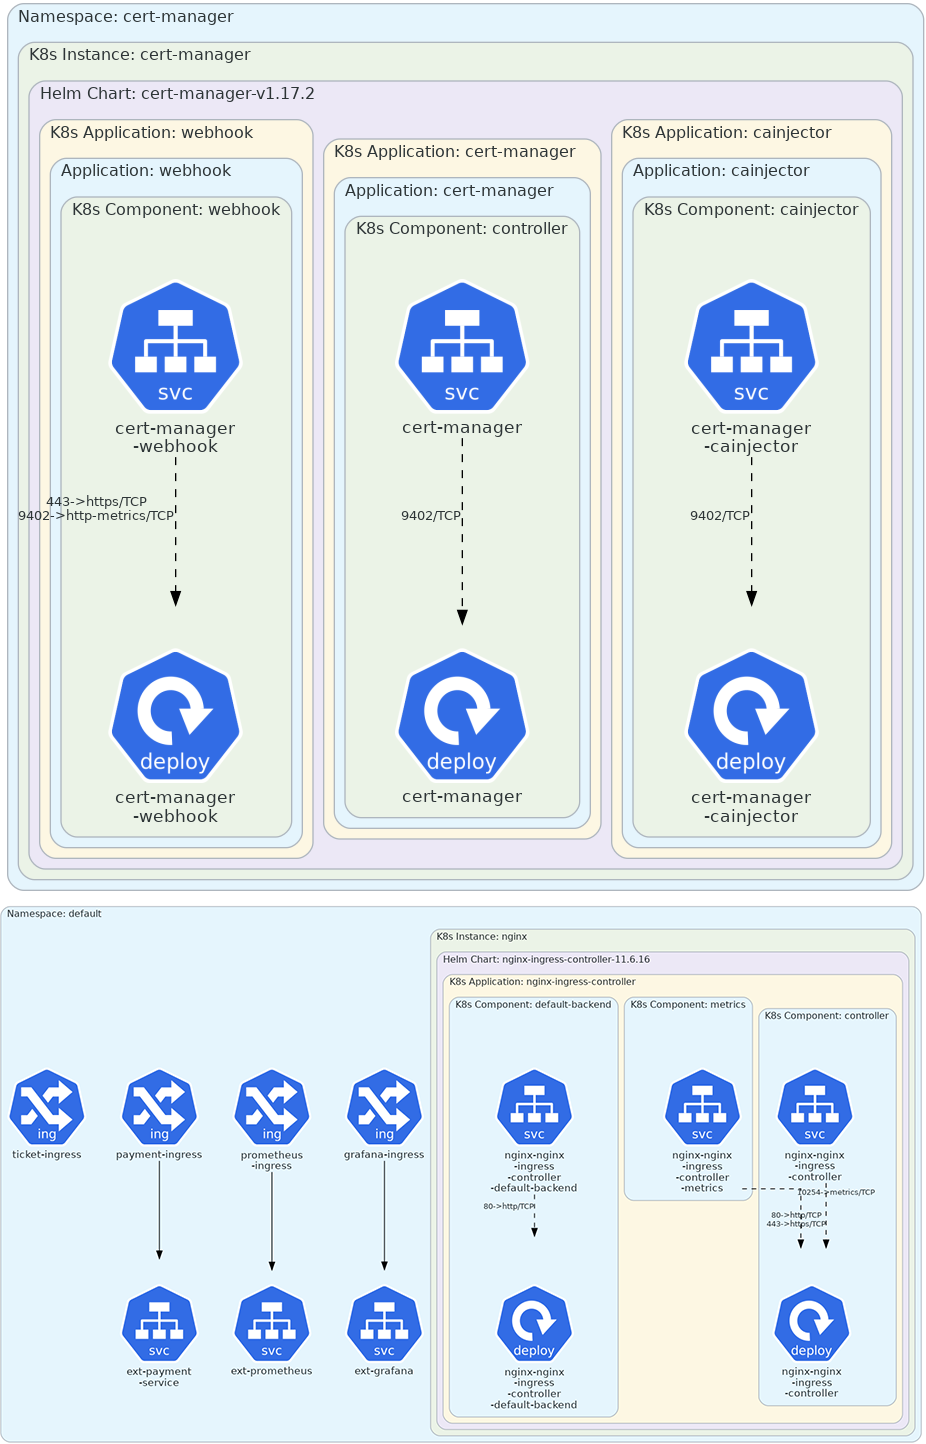
\includegraphics[width=0.75\textwidth]{resources/chapter-4/nginx-1.png}
    \caption{\textit{Deployment} Nginx Ingress}
    \label{fig:deployment-nginx}
\end{figure}

\pagebreak

\subsubsection{Layanan Pembayaran}

Layanan pembayaran secara umum terdiri atas Payment Deployment, Payment Service, dan kluster Redis. Deployment Payment terdiri atas dua kontainer, yaitu Payment Server dan Payment Notifier. Layanan ini digabung dengan kluster sistem tiket untuk mempermudah \textit{deployment}, pengujian, dan memastikan tidak ada masalah jaringan yang terjadi. Diagram \textit{deployment} sistem ini ditunjukkan pada Gambar \ref{fig:deployment-payment}.

\begin{figure}[H]
    \centering
    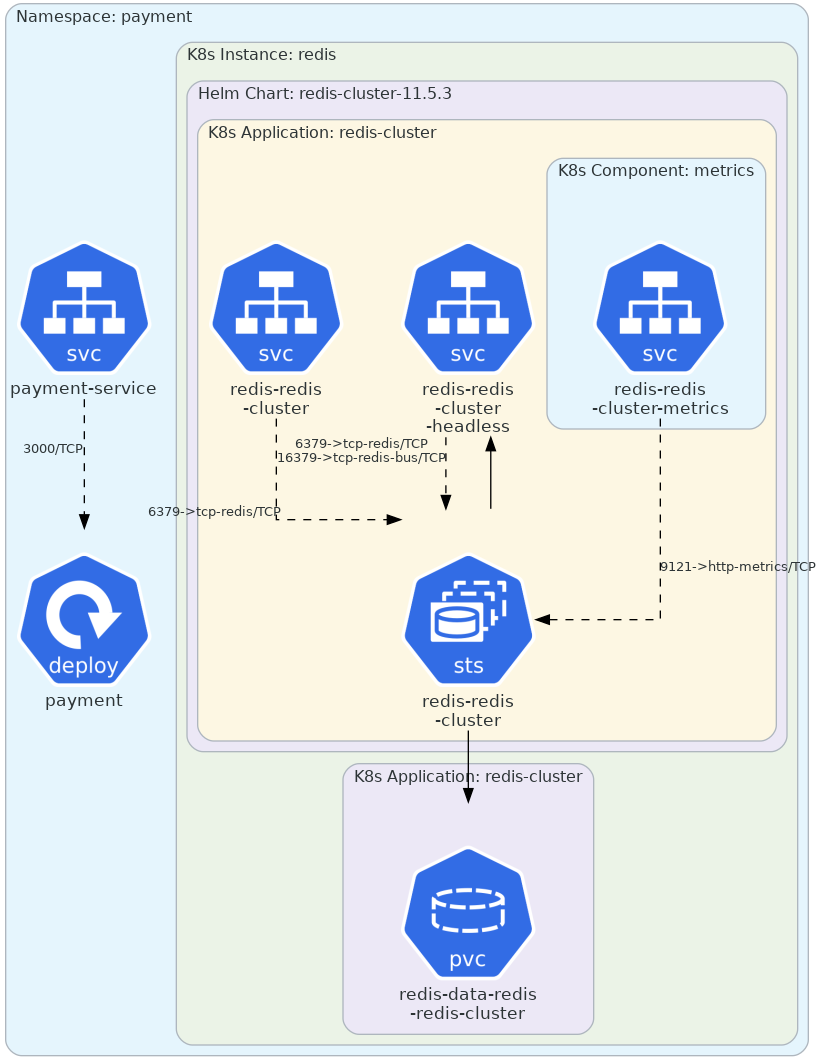
\includegraphics[width=0.8\textwidth]{resources/chapter-4/payment.png}
    \caption{\textit{Deployment} Layanan Pembayaran}
    \label{fig:deployment-payment}
\end{figure}


\pagebreak

\subsubsection{Layanan Tiket tanpa Pengendalian Aliran}

Layanan tiket tanpa pengendalian aliran terdiri atas Ticket Server Deployment, kluster redis, dan Sanity Check Deployment. Sistem ini juga terhubung dengan salah satu kluster basis data relasional yang ada melalui pooler PGCat. Diagram \textit{deployment} sistem ini ditunjukkan pada Gambar \ref{fig:deployment-ticket-nofc}.

\begin{figure}[H]
    \centering
    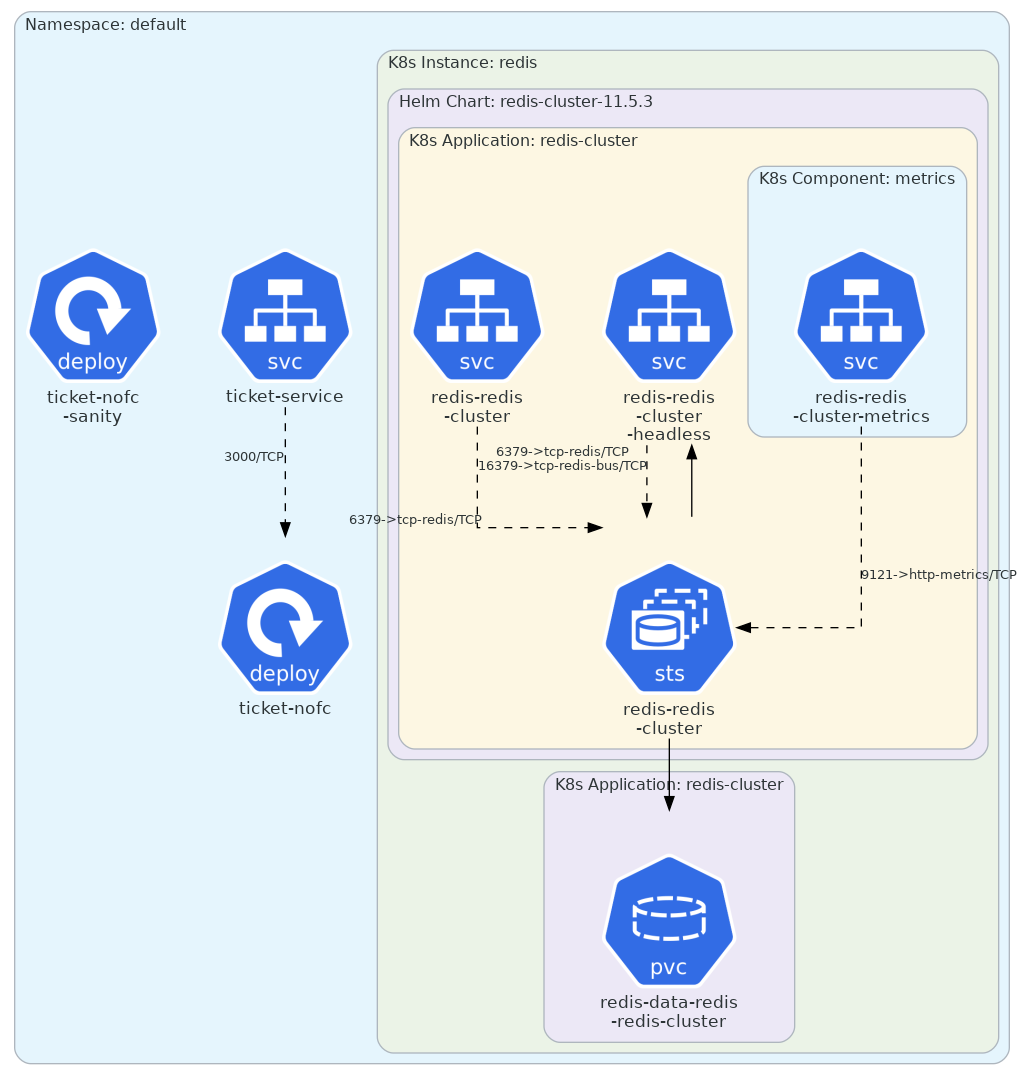
\includegraphics[width=1\textwidth]{resources/chapter-4/ticket-nofc.png}
    \caption{\textit{Deployment} Layanan Ticket tanpa Pengendalian Aliran}
    \label{fig:deployment-ticket-nofc}
\end{figure}

\pagebreak

\subsubsection{Layanan Tiket varian dengan Pengendalian Aliran}

Layanan tiket dengan pengendalian aliran terdiri atas Ticket Server Deployment, Ticket Worker Deployment, kluster redis, RabbitMQ, dan Sanity Check Deployment. Sistem ini juga terhubung dengan salah satu kluster basis data relasional yang ada melalui pooler PGCat. Diagram \textit{deployment} sistem ini ditunjukkan pada Gambar \ref{fig:deployment-ticket-fc}.

\begin{figure}[H]
    \centering
    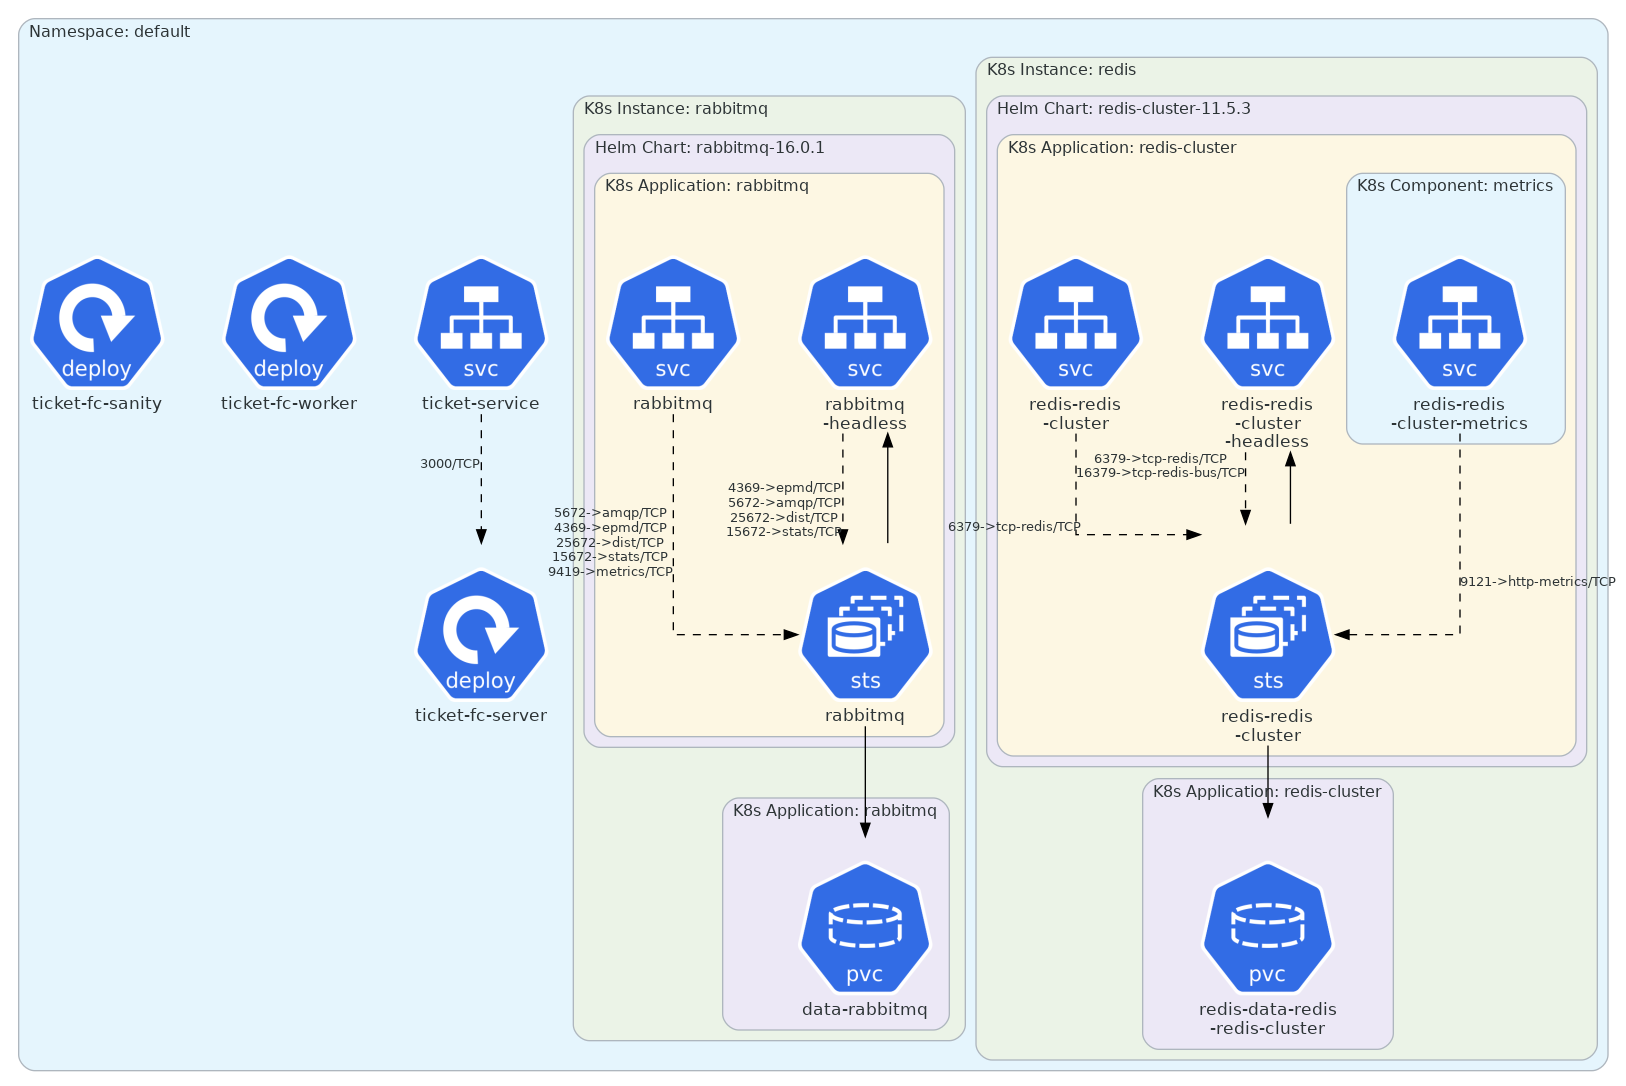
\includegraphics[width=1\textwidth]{resources/chapter-4/ticket-fc.png}
    \caption{Deployment Layanan Ticket dengan Pengendalian Aliran}
    \label{fig:deployment-ticket-fc}
\end{figure}

Hal yang membedakan \textit{deployment} varian ini dengan varian tanpa pengendalian aliran adalah keberadaan kluster RabbitMQ dan Ticket Worker Deployment. Selain itu, program yang dijalankan pada Ticket Server Deployment juga berbeda.

\pagebreak

\subsubsection{Kluster PostgreSQL}

Kluster PostgreSQL terdiri atas PostgreSQL Stateful Set yang akan terdiri atas satu \textit{primary} dan satu replika. Selain itu, terdapat PGCat yang bertindak sebagai pooler dan \textit{load balancer} pada level kueri. PGCat akan membaca kueri dan meneruskan query kepada \textit{primary} atau replika berdasarkan jenis kueri dan beban setiap instans. Diagram \textit{deployment} sistem ini ditunjukkan pada Gambar \ref{fig:deployment-postgres}.

\begin{figure}[H]
    \centering
    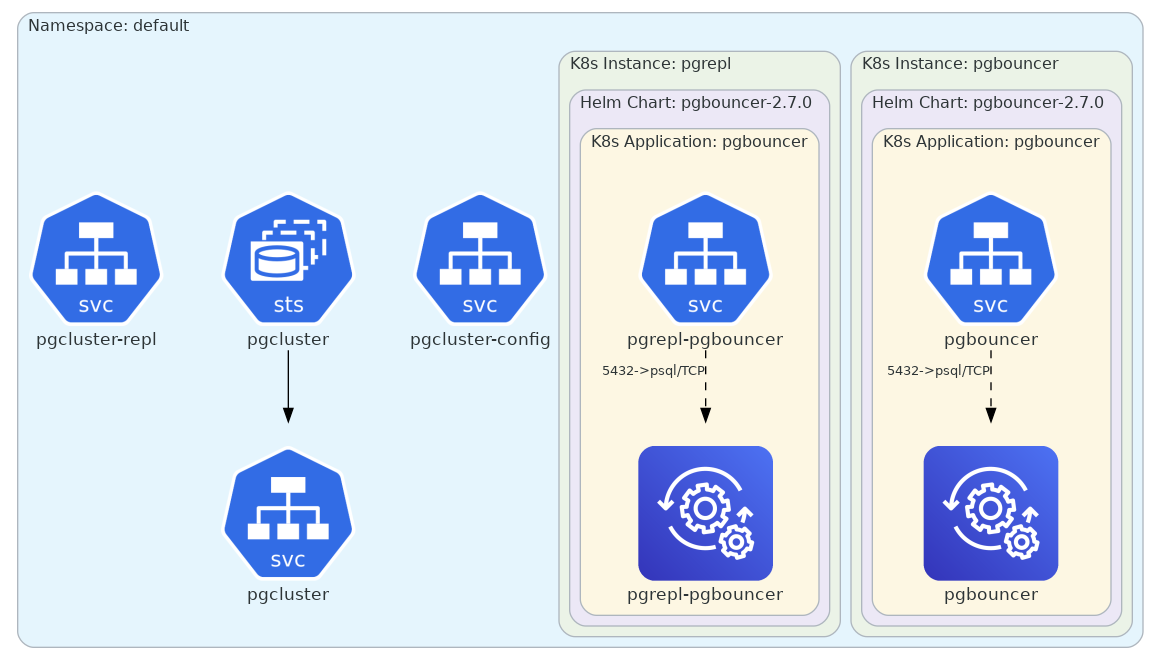
\includegraphics[width=1\textwidth]{resources/chapter-4/postgres.png}
    \caption{Deployment kluster PostgreSQL}
    \label{fig:deployment-postgres}
\end{figure}


\pagebreak

\subsubsection{Kluster CitusData}

Kluster CitusData terdiri atas tiga CitusCluster Stateful Set. Kluster pertama merupakan koordinator dan sisanya merupakan pekerja. Terdapat PGCat yang terhubung dengan koordinator. Sistem tiket terhubung langsung dengan PGCat. Koneksi dengan pekerja dilakukan melalui koordinator. Diagram \textit{deployment} sistem ini ditunjukkan pada Gambar \ref{fig:deployment-citusdata}.

\begin{figure}[H]
    \centering
    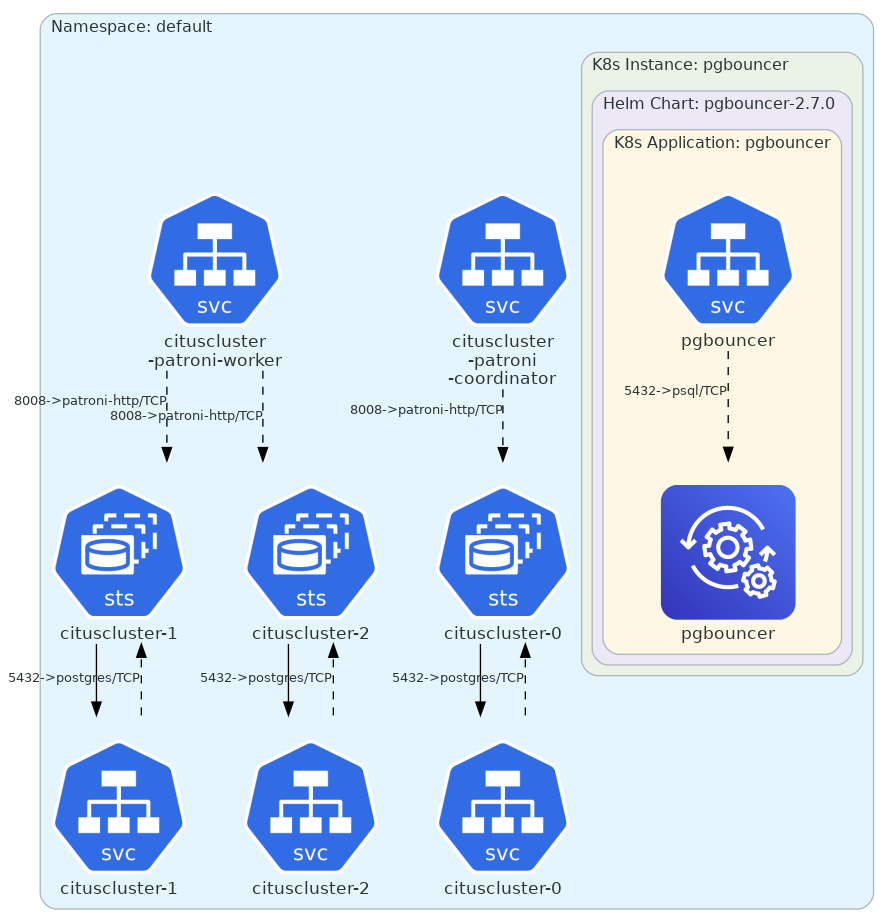
\includegraphics[width=1\textwidth]{resources/chapter-4/citusdata.png}
    \caption{Deployment kluster CitusData}
    \label{fig:deployment-citusdata}
\end{figure}

\pagebreak

\subsubsection{Kluster YugabyteDB}

Kluster YugabyteDB terdiri atas YB-Master Stateful Set, YB-TServer Stateful Set, dan PGCat. PGCat terhubung dengan semua instans YB-TServer. Sistem tiket terhubung langsung dengan PGCat. Proses \textit{load balancing} koneksi dengan YB-TServer ditangani oleh PGCat. Diagram \textit{deployment} sistem ini ditunjukkan pada Gambar \ref{fig:deployment-yugabyte}.

\begin{figure}[H]
    \centering
    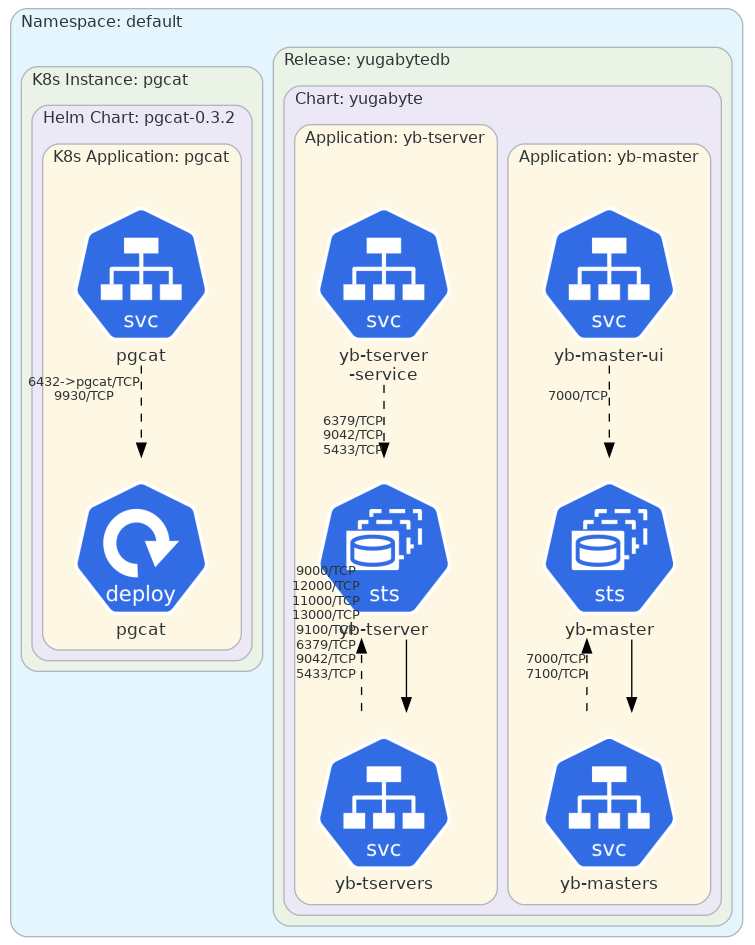
\includegraphics[width=1\textwidth]{resources/chapter-4/yugabyte.png}
    \caption{Deployment kluster YugabyteDB}
    \label{fig:deployment-yugabyte}
\end{figure}

\pagebreak

\subsection{Konfigurasi \textit{Deployment} Kluster Agen Penguji}

\subsubsection{Sistem Pengawasan}

Sistem pengawasan pada agen penguji lebih sederhana dengan komponen pengawasan hanya terdiri atas Grafana Dashboard dan Prometheus. Grafana Alloy dan Loki tidak digunakan karena \textit{log} yang relevan hanya berasal dari eksekusi K6 yang isinya dapat ditampilkan dengan perintah tertentu. Selain itu, hal ini dilakukan untuk mengurangi penggunaan sumber daya yang tidak perlu, sehingga besarnya sumber daya yang dapat digunakan untuk K6 menjadi lebih banyak. Diagram \textit{deployment} sistem ini ditunjukkan pada Gambar \ref{fig:deployment-monitoring-agent}.

\begin{figure}[H]
    \centering
    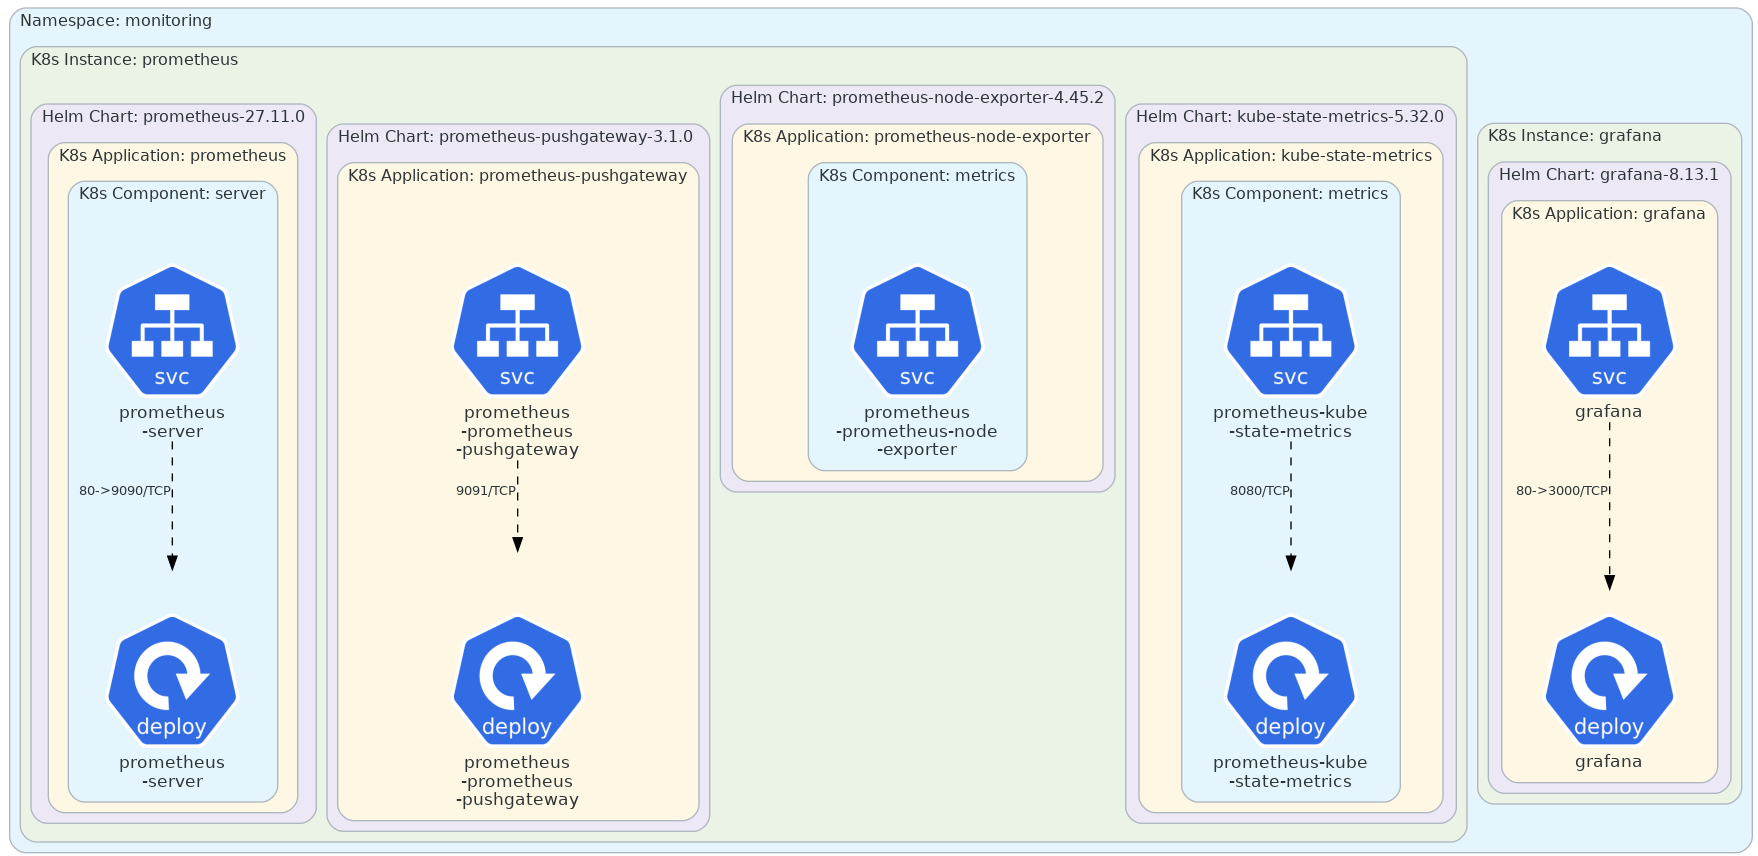
\includegraphics[width=1\textwidth]{resources/chapter-4/agent-monitoring.png}
    \caption{\textit{Deployment} Sistem Monitoring}
    \label{fig:deployment-monitoring-agent}
\end{figure}

\subsubsection{Nginx Ingress Controller}

Komponen ini memiliki \textit{deployment} yang sama seperti klsuter sistem tiket sebagaimana ditunjukkan pada Gambar \ref{fig:deployment-nginx}. Hanya saja, perbedaannya terletak pada tidak adanya \textit{ingress} layanan tiket dan layanan pembayaran.

\pagebreak

\subsubsection{K6 Operator}

K6 Operator merupakan komponen utama kluster penguji. Komponen ini mengatur inisiasi dan \textit{runtime} kode pengujian k6. Saat pengujian dijalankan, Grafana Operator akan menginisiasi instans K6 sebanyak 12 instans. Instans ini akan didistribusikan ke berbagai node pada kluster. Diagram \textit{deployment} sistem ini ditunjukkan pada Gambar \ref{fig:deployment-k6-operator}.

\begin{figure}[H]
    \centering
    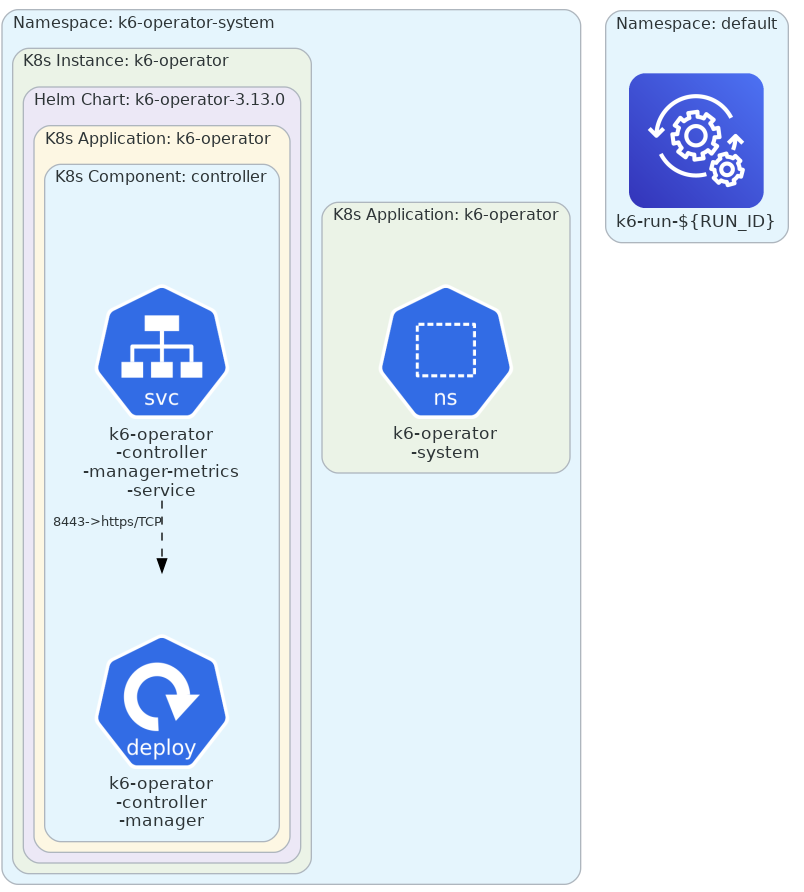
\includegraphics[width=1\textwidth]{resources/chapter-4/k6-operator.png}
    \caption{Deployment K6 Operator}
    \label{fig:deployment-k6-operator}
\end{figure}

\pagebreak